\section{Experimentbeschreibungscode}
\lstinputlisting{code/experiment.edl}
\begin{code}[H]
    \caption{EDL-Experimentbeschreibungscode}
    \label{code:edl-experimentbeschreibungscode}
\end{code}

\section{Modellbeschreibungscode}
\lstinputlisting{code/ausgangspunkt.mdl}
\begin{code}[H]
	\caption{MDL-Modellbeschreibungscode}
	\label{code:mdl-modellbeschreibungscode}
\end{code}

\twocolumn

\newpage

\begin{figure}[H]
    \subfloat[Medium: Luft]{\includegraphics[width=0.88\linewidth]{Dichte/Luft/map}}\\
    \subfloat[Medium: Wolframhexafluorid]{\includegraphics[width=0.88\linewidth]{Dichte/Wolframhexafluorid/map}}\\
    \subfloat[Medium: Wasser]{\includegraphics[width=0.88\linewidth]{Dichte/Wasser/map}}
    \caption{Fraktalbilder bei veränderter Dichte des Mediums}
    \label{fig:Fraktalbilder_bei_veränderter_dichte_des_mediums}
\end{figure}

\begin{figure}[H]
    \subfloat[Pendelmasse: $0.04 kg$]{\includegraphics[width=0.88\linewidth]{Masse/0.04/map}}\\
    \subfloat[Pendelmasse: $0.02 kg$]{\includegraphics[width=0.88\linewidth]{Masse/0.02/map}}\\
    \subfloat[Pendelmasse: $0.01 kg$]{\includegraphics[width=0.88\linewidth]{Masse/0.01/map}}
    \caption{Fraktalbilder bei veränderter Pendelmasse}
    \label{fig:Fraktalbilder_bei_veränderter_pendelmasse}
\end{figure}

\begin{figure}[H]
    \subfloat[Magnetladung: $1 \cdot 10^{-7} C$]{\includegraphics[width=0.88\linewidth]{Magnetladung/1E-7/map}}\\
    \subfloat[Magnetladung: $4 \cdot 10^{-7} C$]{\includegraphics[width=0.88\linewidth]{Magnetladung/4E-7/map}}\\
    \subfloat[Magnetladung: $4 \cdot 10^{-6} C$]{\includegraphics[width=0.88\linewidth]{Magnetladung/4E-6/map}}
    \caption{Fraktalbilder bei veränderter Magnetstärke}
    \label{fig:Fraktalbilder_bei_veränderter_magnetstärke}
\end{figure}

\begin{figure}[H]
    \subfloat[Standort: Jupiter]{\includegraphics[width=0.88\linewidth]{Erdbeschleunigung/Jupiter/map}}\\
    \subfloat[Standort: Erde]{\includegraphics[width=0.88\linewidth]{Erdbeschleunigung/Erde/map}}\\
    \subfloat[Standort: Schwerelosigkeit]{\includegraphics[width=0.88\linewidth]{Erdbeschleunigung/Schwerelosigkeit/map}}
    \caption{Fraktalbilder bei veränderter Fallbeschleunigung}
    \label{fig:Fraktalbilder_bei_veränderter_fallbeschleunigung}
\end{figure}

\newpage